\chapter{Introduction}
\label{cha:Introduction}

FPGAs offer the flexibility to design application specific hardware
for different kinds of computational intensive problems. They are capable
of providing high memory bandwidths by using wide data buses and pipelines.
As the are reconfigurable, reusing them for different kinds of problems
is easy and does not add huge overheads. Such benefits have increased
the popularity of the FPGA based accelerators as an alternative to the
GPUs in a heterogenous \ac{HPC}.
A High performance cluster contains multiple individual
systems known as nodes. Each node can contain multiple multi-core processors,
along with accelerators such as GPUs and FPGAs. The nodes are connected to each other
using high speed interconnects to exchange data and control information. The whole system acts
as a single high performance system with distributed memory and processing elements as
shown in Figure \ref{fig:cluster}. The applications run parallely on multiple cluster node
and utilize the high speed interconnects to communicate and exchange data. Using
multiple nodes with the FPGA/GPU accelerators allow to speedup the execution by use of more computing resources.
\begin{figure}[ht]%
    \centering
    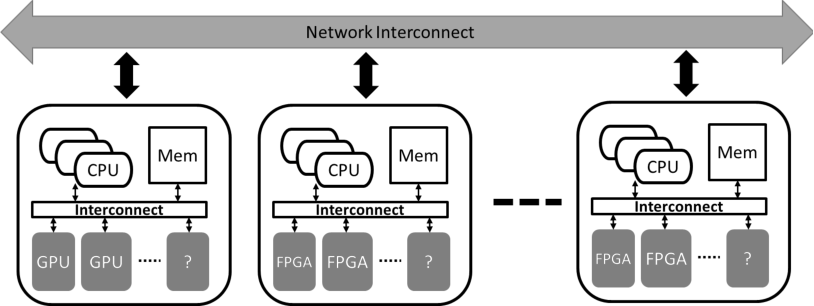
\includegraphics[width=1.0\textwidth]{images/cluster}
    \caption{High performance cluster structure with multiple nodes having different configuration}
    \label{fig:cluster}
\end{figure}

The FPGA based accelerators in the nodes are mostly used to implement mathematical computations such
as matrix multiplication, fast fourier transformation and string manipulation which form the
basis for most of the application. Using the FPGA's features such as data and instruction pipelining,
replication and memory localization, the FPGAs can be used to decrease the execution time of
these mathematical operations. Increasing popularity of the FPGAs in the high performance
computing has led to new innovations for the FPGAs. Higher memory bandwidths, increased count
of logical units and bigger local memory are some of these. Also, alternative hardware design development
flows and tools are now used such as OpenCL which provide a C/C++ based design flow for
the FPGAs. The OpenCL design flow is simpler and abstracts the complex hardware design
challenges from a typical user of the High performance computing cluster making
the application development with the FPGA accelerators simple.

To utilize the benefits of the FPGA accelerators, the new Noctua \ac{HPC} cluster at Paderborn Center for
Parallel Computing (PC\textsuperscript{2}) contains 32 BittWare 520N
FPGA accelerator boards having Intel Stratrix 10 FPGAs. Apart from having the high performance FPGA, the BittWare 520N boards
are also equipped with four 100/40/25/10G QSFP28 network ports. These Network ports can be used as
high speed serial IO channels to set up communication infrastructure between the FPGAs.
Using the ports, the dependency of the FPGA on the CPUs for communicating
the data can be removed. The high speed communication setup between the FPGAs can be used to scale
up application over multiple FPGAs with small communication latency freeing the CPU
to perform additional computation simultaneously.

MIDG2\footnote{\url{https://github.com/tcew/MIDG2}} is an \ac{MPI} based parallel computation
implementation of the \ac{DG} \cite{hesthaven_nodal_2008} method to solve Maxwell’s equation
in time domain. \ac{DG} method is a commonly used operation in many simulation applications to
solve \ac{PDE} and improvements to the computation time would be an important step to
benefit different simulation applications utilizing this method. This thesis presents
a design which evaluates the benefits of using a parallel distributed FPGA based system
to reduce the execution time of the application by using direct FPGA-to-FPGA communication.

\section{Objectives}

Noctua \ac{HPC} cluster equipped with FPGAs provides opportunities to create applications
which are accelerated with multiple FPGAs. As there is
no known implementation utilizing FPGA in network configuration for accelerating the
DG method, this master thesis aims at presenting such a system to evaluate
the achievable acceleration with multiple FPGAs using point-to-point communication in
different network topologies for the MIDG2 application. Towards achieving this target,
the evaluation can be divided into two stages. First stage aims at identifying
and evaluating the possible topologies for point-to-point communication. In the second
stage of the thesis, the existing OpenCL based FPGA implementation for
the MIDG2 application would be extended to use IO channels.

Considering the two stages as individual sub-tasks, the first task involves building
prototypes using OpenCL IO channels which would utilize the four 100/40/25/10G QSFP28
network ports available on the BittWare 520N boards. These prototypes would be used
to evaluate the point-to-point topologies using bandwidths and latency to give an
overview of possible benefits. The prototypes would also serve as the basis for
understanding the implementation opportunities available in the OpenCL and
BittWare BSP for the channels. The second task would be then to utilize the
understanding and extend the OpenCL kernels for the MIDG2 application
such that the need for \ac{MPI} communication to communicate information or the shared
surfaces is eliminated and overheads are removed.

\section{Related Work}

\ac{DG} method is believed to be first proposed by \textcite{reed_triangular_1973} for
solving the steady-state neutron transport equation \cite{hesthaven_nodal_2008}. Over the
years many researchers have proven the accuracy of the method and developed improvements
over the original method to use in different fields for solving \ac{PDE}. The \ac{DG} method
is popular today to solve equations in the fields of acoustics \cite{wilcox_high-order_2010,
atkins_quadrature-free_1998, toulopoulos_high-order_2006}, elasticity \cite{dumbser_arbitrary_2006,
kaser_arbitrary_2006, kaser_arbitrary_2007}, electrodynamics Maxwell’s equation \cite{busch_discontinuous_2011,
cohen_discontinuous_2006, busch_discontinuous_2011, cohen_spatial_2006, cockburn_locally_2004,
konig_discontinuous_2010} and thermodynamics \cite{collis_discontinuous_2002}.

The popularity of the \ac{DG} method has led researchers to develop parallel methods
which can speed up the application to reduce the execution time. As the DG method
performs operations on local elements followed by accumulation, this allows parallelization
of the operations on elements and has been utilized to create various parallel systems.
\textcite{baggag_parallel_1999} presents a parallel system which is used to simulate aeroacoustic
scattering and uses \ac{MPI} data exchange. \textcite{klockner_nodal_2009} showed the benefits
of using GPU for accelerating the computation by utilizing the capability of the GPU to
process data in parallel. They use CUDA programming for GPUs to get improved memory bandwidths
and higher computation efficiency. \textcite{bernacki_parallel_2006} discuss the benefits
of parallelization achieved by partitioning the tetrahedral meshes for realistic problems
involving electromagnetic wave radiation study for different objects. Though the use of such
parallel architecture and use of GPU based accelerators have proven
to improve the simulation time, they often require large data sets to show the benefits of
such improvements.

FPGAs based accelerators utilize techniques such as efficient arithmetic operations using DSPs,
deep instruction and pipelining to decrease computation time, multiple compute units for
large scale parallel computations.
Such benefits have made FPGAs a popular choice for implementing accelerators for
problems utilizing heavy floating point computation. Considering such benefits,
an implementation for accelerating the \ac{DG} operations in FPGAs was
developed by \textcite{kenter_opencl-based_2018}. The implementation shows the benefit
of using a single FPGA over a highly parallelized multi-core CPU implementation for
the MIDG2 application which solves Maxwell’s equations in time domain. While working at
PC\textsuperscript{2}, I implemented an extension of this design before the start of this thesis
which is capable of using multiple single FPGAs to scale the application to 32 FPGAs using
communication via CPU. This design is used as the base for this thesis.

The increased popularity of the FPGAs in past has led to identify possibilities for
using multiple FPGAs. This can be achieved by using \ac{MPI} communication via the CPU host
to which the FPGA is connected. Though such design posses benefits in many cases,
it performs poorly in case of multiple and large transfer due to low bandwidths
and higher latency for the PCIe + \ac{MPI} combination \cite{kobayashi_opencl-ready_2018}.
Systems have been investigated where the FPGAs could
communicate directly without the need of host. \textcite{sheng_hpc_2017} presents a design
for 3D FFT solver which uses a 3D-torus FPGA-based network using a table-based routing
scheme. The evaluation results of such design shows 30\% improvement over the reference design.
\textcite{kobayashi_opencl-ready_2018} used an OpenCL based design implementation to
compare the latency of \ac{MPI}+PCIe based system and FPGA-to-FPGA system which uses Ethernet
IP for communication over an switch. The results show a large difference between the achievable
bandwidths and latency for the two system proving the benefits of such system. The system
design presented in this thesis uses a similar approach like in \cite{kobayashi_opencl-ready_2018}
but does not utilize the Ethernet-IP core and relies on the serial communication
support provided in the BittWare BSP.

The rest of the thesis is divided into 5 chapters. Chapter \ref{cha:Fundamentals} discusses
the fundamentals components and technologies used in the thesis giving details of the DG method
and and overview of the OpenCL application development and techniques. It also introduces
the single FPGA design presented in \cite{kenter_opencl-based_2018} and the distributed
version using multiple FPGAs. Chapter \ref{cha:topologies} introduces the topologies which
are possible for the FPGAs along with the prototypes developed. The chapter also presents
the results of the evaluation of the topologies with synthetic data. Chapter \ref{cha:sys_arch}
gives details of the first implementation done using IO channels describing
the changes in OpenCL kernels. Chapter \ref{cha:sys_fpgaonly}
presents the \texttt{FPGA only} system implemented by optimizing the IO channels design
to remove the host dependency in the kernels. It also discusses the issues faced while
optimizing the OpenCL kernels. Chapter \ref{cha:Evaluation} discusses the evaluation steps
and the results of the evaluation comparing the design variants. It also presents a detailed
analysis of the results to highlight the bottlenecks in the design.
Final chapter \ref{cha:Conclusion} presents a conclusion of the achieved results of the thesis
and proposes possible future works and improvements.